\documentclass{beamer}

%\usetheme{Madrid}
%\usetheme{Boadilla}
%\usetheme{default}
%\usetheme{Warsaw}
%\usetheme{Bergen}
%\usetheme{Frankfurt}
\usetheme{Darmstadt}

\setbeamercolor{normal text}{fg=white}
\setbeamertemplate{background canvas}[vertical shading] [top=black!95,bottom=black!65]

\definecolor{mypurple}{RGB}{207,78,64}
\usecolortheme[named=mypurple]{structure}

\definecolor{myorange}{RGB}{255,235,190}
\beamerboxesdeclarecolorscheme{orange}{orange}{myorange}

\definecolor{commandcolor}{RGB}{111,195,165}

\setbeamertemplate{footline}[page number]
%\setbeamercovered{transparent}
\setbeamercovered{invisible}
\setbeamertemplate{navigation symbols}{}

%\usepackage{musixtex}
\usepackage{multimedia}
\usepackage{graphicx}
\usepackage[utf8]{inputenc}
%\usepackage[T1]{fontenc}
\usepackage[french]{babel} 
%\usepackage[all]{xy}
%\usepackage{multirow}
%\usepackage{lmodern}
\usepackage{subfigure}
%\usepackage{ulem}
\usepackage{url}
\usepackage{hyperref}
\usepackage{verbatim}
\usepackage{xspace}
\usepackage{color}
\usepackage{xcolor}
\usepackage{rotating}
\usepackage{multicol}
\usepackage[export]{adjustbox}
\usepackage{textpos}
\usepackage{listings}
\usepackage{fontawesome}


\definecolor{mypurple}{RGB}{207,78,64}
\usecolortheme[named=mypurple]{structure}

\definecolor{myorange}{RGB}{255,235,190}
\beamerboxesdeclarecolorscheme{orange}{orange}{myorange}

\definecolor{dgreen}{RGB}{0,125,0}

\usepackage{tikz}
\usetikzlibrary{trees}

\setbeamertemplate{caption}[numbered] 

\newcommand{\setframetitle}[1]{\begin{center}
    \huge \textbf{#1}
\end{center}}


%% --------------

\title{Gitlab}
\subtitle{Atelier d'aide à la programmation}
\author{L\'eo \textsc{Baudouin}}
\institute{
  {\url{baudouin.leo @ gmail.com}}
}
\date{03-04 juin 2019}

%% --------------

\begin{document}

\begin{frame}
  \titlepage
\end{frame}

\section{Introduction}
\subsection{}

\begin{frame}{Définition}


\begin{center}

\includegraphics[width=0.5\linewidth]{images/gitlab-logo}
\end{center}

\begin{block}{Wikipedia}
{\it 
«~GitLab est un logiciel libre de forge basée sur git proposant les fonctionnalités de wiki, un système de suivi des bugs, l’intégration continue et la livraison continue....}
\end{block}
\end{frame}



\begin{frame}[fragile]{Gitlab}

\begin{block}{Online}
\href{https://gitlab.com}{https://gitlab.com}
\end{block}

\begin{block}{Installation locale}
\scriptsize
\begin{verbatim}
docker run -d --name gitlab --restart always gitlab/gitlab-ce:latest
\end{verbatim}
\end{block}


\end{frame}



\section{Intégration Continue}
\begin{frame}[fragile]{Intégration Continue}

\begin{block}{.gitlab-ci.yml}
\begin{verbatim}
image: lbaudouin/latex

build:
  script:
    - latexmk -pdf
  artifacts:
    paths:
      - "*.pdf"
    expire_in: 2 year
\end{verbatim}
\end{block}

Résultat:
\footnotesize
\href{https://gitlab.com/lbaudouin/cv/-/jobs/artifacts/master/raw/cv-lbaudouin.pdf?job=build}{https://gitlab.com/\textbf{user}/\textbf{project}/-/jobs/artifacts/master/raw/\textbf{file}?job=\textbf{job}}

\end{frame}



\begin{frame}[fragile]{CI}
\begin{block}{Pipeline}
\begin{center}
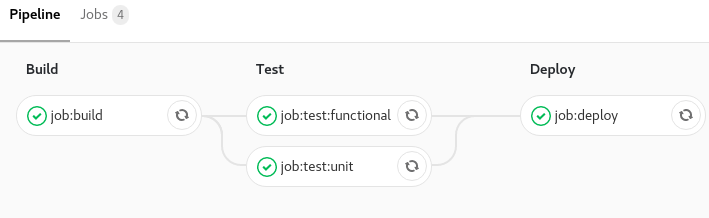
\includegraphics[width=1.0\linewidth]{images/ci-stages}
\end{center}
\end{block}
\end{frame}




\begin{frame}[fragile]{CI}

\begin{block}{.gitlab-ci.yml}
\scriptsize
\begin{verbatim}
build:
  stage: build
  script: make build

test:unit:
  stage: test
  script: make test-unit

test:functional:
  stage: test
  script: make test-functional

deploy:
  stage: deploy
  script: make deploy
\end{verbatim}
\end{block}
\end{frame}





%-------------------------------------------------------------------

\end{document} 
